%%%%%%%%%%%%%%%%%%%%%%%%%%%%%%%%%%%%%%%%%
% Masters/Doctoral Thesis 
%
% Template license:
% CC BY-NC-SA 3.0 (http://creativecommons.org/licenses/by-nc-sa/3.0/)
%
%%%%%%%%%%%%%%%%%%%%%%%%%%%%%%%%%%%%%%%%%

% https://www.overleaf.com/latex/templates/template-for-a-masters-slash-doctoral-thesis/mkzrzktcbzfl#.Wj_WWFT1VPW

%----------------------------------------------------------------------------------------
%   Кофигуриране на пакети и опции.
%----------------------------------------------------------------------------------------

\documentclass[12pt,bulgarian,singlespacing,headsepline,oneside,openany]{thesis}

% Използване на UNICODE.
\usepackage{ucs}
\usepackage[utf8x]{inputenc}

% Рефериране на думи и други обекти.
\usepackage{nameref}

% Рефериране на хипер връзки.
\usepackage{hyperref}

% Кодировка за международни езици.
\usepackage[T1]{fontenc}

% ???
\usepackage{url}

% ???
\usepackage{lipsum}

% Използване на графика.
\usepackage{graphicx}

% Директория в която се намират изображенията.
\graphicspath{{images/}}

% ???
\usepackage{array}

% Автоматично създаване на различните индекси.
\usepackage{imakeidx}

% ???
\usepackage{placeins}

% Възможност за включване на форматиран програмен код.
\usepackage{listings}

% За списъка със съкращенията.
\usepackage[acronym]{glossaries}
\makeglossaries
\newacronym{rdms}{СУБД}{система за управление на бази от данни}

% Автоматично създаване на азбучен указател.
\makeindex[columns=1, title=Азбучен указател, intoc]

%----------------------------------------------------------------------------------------
%   Настройки на страницата.
%----------------------------------------------------------------------------------------

\geometry{
	% Размер на листа.
	paper=a4paper,
	% Вътрешно отместване.
	inner=2.5cm,
	% Външно отместване.
	outer=3.8cm,
	% Отместване за свързване.
	bindingoffset=.5cm,
	% Отместване от горния край.
	top=1.5cm,
	% Отместване от долния край.
	bottom=1.5cm, 
	% Рамка на самата страница.
	%showframe,
}

%----------------------------------------------------------------------------------------
%   Данни за дисертацията.
%----------------------------------------------------------------------------------------

% Заглавие на дисертацията.
\thesistitle{Клиент-сървър игра на дъска за мобилни устройства}

% Вид на научната степен.
\degree{"Магистър"} 

% Имена на автора.
\author{\href{https://www.linkedin.com/in/boyana-kantarska-9b1363a3/}{Бояна Радкова \textsc{Кантарска}}}

% Вид на научната степен.
\supervisor{ас. Делян Керемедчиев} 

% Служебен адрес.
\addresses{НБУ, ул. Монтевидео 21, София 1618, България} 

% Научна област.
\subject{MSNINF01 "Софтуерни технологии в Интернет"} 

% Ключови думи.
\keywords{} 

% Учебно заведение.
\university{\href{http://www.nbu.bg}{Нов български университет}}

% Подразделение.
\faculty{\href{http://nbu.bg/bg/fakulteti/magistyrski-fakultet}{"Магистърски факултет"}} 

% Работна група.
\department{\href{http://computerscience.nbu.bg}{"Информатика"}}

% Параметри на генерирания PDF файл.
\AtBeginDocument{
% Заглавие на PDF файла.
	\hypersetup{pdftitle=\ttitle}
% Автор на PDF файла.
	\hypersetup{pdfauthor=\aname}
% Ключови думи на PDF файла.
	\hypersetup{pdfkeywords=\keywordnames}
}

%----------------------------------------------------------------------------------------
%   Начало на същинския документ.
%----------------------------------------------------------------------------------------

\begin{document}

% Използване на римска номерация за страниците предхождащи същинското изложение.
\frontmatter

% Изчистване на стила за страницата преди да започне същинското изложение.
\pagestyle{plain}

%----------------------------------------------------------------------------------------
%   Заглавна страница.
%----------------------------------------------------------------------------------------

\begin{titlepage}
\begin{center}

\vspace*{.01\textheight}

% Название на учебното заведение.
{\scshape \LARGE 
% Лого на университета.

\includegraphics[width=0.08\linewidth]{nbu_logo}
\univname \\[0.5cm] 
% Лого на департамента.
%
\includegraphics[width=0.1\linewidth]{nbu_logo}
\facname \\[0.5cm] 
\deptname \par}

\vspace{1.5cm}
 
% Автор.
\aname

\vspace{1.5cm}

% Хоризонтална линия.
\HRule \\[0.4cm]

% Заглавие на дисертацията.
{\large \bfseries \ttitle \par}\vspace{0.4cm}

% Хоризонтална линия.
\HRule \\[1.5cm]

% Вид документ.
\textsc{\Large МАГИСТЪРСКА ТЕЗА}\\[0.5cm] 
 
\vfill

% Текст изискван от учебното заведение.
\large \textit{за степен \degreename}\\[1.3cm]

%Област на тезата.
\subjectname \vspace{1.5cm}
 
\vfill

Ръководител: \supname
 
\vfill
 
% Година на предаване.
{\large София \\ 2019}
 
\vfill
\end{center}
\end{titlepage}

%----------------------------------------------------------------------------------------
%   Декларация за достоверност.
%----------------------------------------------------------------------------------------

\begin{declaration}

\vspace{2cm}

Декларирам, че настоящата теза съдържа оригинални резултати, получени при проведените от мен научни изследвания. Резултатите, които са получени, описани и/или публикувани от други учени, са надлежно и подробно цитирани в библиографията.

\vspace{0.5cm}

Настоящата теза не е представяна в процедури за придобиване на научна степен в друго висше училище, университет или научен институт.

\vspace{2cm}

\hspace{4cm}
Подпис: 

\vspace{0.25cm}

\hspace{5cm}
/ \aname /
\end{declaration}

%----------------------------------------------------------------------------------------
%   Таблицата на съдържанието.
%----------------------------------------------------------------------------------------

\newpage
\tableofcontents

%----------------------------------------------------------------------------------------
%   Списък с абревиатурите.
%----------------------------------------------------------------------------------------

\printglossary[type=\acronymtype,title={Списък с абревиатурите}]

%----------------------------------------------------------------------------------------
%   Списък с фигурите.
%----------------------------------------------------------------------------------------

\newpage
%\listoffigures

%----------------------------------------------------------------------------------------
%   Списък с таблиците. 
%----------------------------------------------------------------------------------------

\newpage
%\listoftables

%----------------------------------------------------------------------------------------
%   Основно изложение организирано в глави.
%----------------------------------------------------------------------------------------

% Номерация с арабски цифри за същинската част на дисертацията.
\mainmatter

% Оформление в стил на дисертация.
\pagestyle{thesis}

% По този начин номерацията на подточките е с арабски цифри.
\renewcommand\thesection{\thechapter.\arabic{section}}
\renewcommand\thesubsection{\thesection.\arabic{subsection}}

\newpage
\chapter{Обзор на игрите}
\label{chapter01}

“Stratego” представлява логическа игра характеризираща се с абстракцията, която от своя страна поражда аналитичното мислене в играчите. Логическите игри добиват наименование си поради структурата си, която се гради на точно определени правила създаващи интересни сценарий за играчите. Под формата на въпроси, екстремни тестове, задачи и други способи, като сравняваща оценка между участниците и това как реагират и действат в динамична ситуация. Текущите логически игри са разнообразни. По принцип всяка логична задача може да бъде "gamified" (да прилагат типични елементи на игра (например точкуване, съревнование с противника, правила на игра) към (дейност), обикновено като онлайн маркетингова техника за насърчаване на ангажираността с продукт или услуга), чието динамично взаимодействие тества основната идеята. 

\section{История на логическите игри}

\begin{lstlisting}
https://en.wikipedia.org/wiki/Logic_games
\end{lstlisting}

Логическите игри се разделят на няколко типа, които обстойно изучават семантиката и конструкцията и. Основният е линейният, тъй като съдържа два асортимента от променливи. Те наслояват променливите като ги съпоставят една с друга съгласно инструкциите на дадената игра. Следващият тип - разширено линеен е сходен на предходния, но броят на променливи се увеличава започвайки от три или повече променливи. При груповият вид концепцията се отклонява от стандартната,променливите са присвоени на групи като не се спазва определена последователност. Последният вид е съчетание между груповите и променливите.

Логическите игри биват характеризирани като специфични, тъй като следят разсъжденията и поведението на играчите в напрегната и несигурна ситуация, което прави играта по реалистична като изживяване, а на теория обогатява знанията и разширява гледната точка на участниците.

\subsection{Игри с открити условя}

Най-сериозните игри са с перфектна информация. Перфектната информация означава, че всеки път, когато един от играчите прави ход, който зависи от избора му на стратегия той знае всички минали ходове на играта, включително и шансовете. Например шахът е игра с перфектна информация, тъй като всеки играч може да вижда фигурите на противника по всяко време. 

Игрите с перфектна информация имат особено проста математическа структура. Всяка игра от типа на перфектна информация, се свежда до оптимални стратегически ходове от двамата играчи, който взимат крайни решения спрямо информацията придобита по време на игра. Основната теорема е на Кун през 1953г., която гласи, че при крайни игри с перфектно информация, всяко разпределение чрез смесени стратегии, е постижимо и чрез поведенчески стратегии.

Въпреки това, "игра с пълна информация" понякога включва игри като Табла или Монополи, които въпреки че имат случайни събития (хвърляне на зарове), те не съдържат все още нямат информация, която е известна като в шаха. Вероятностите за всички случайни събития трябва да бъдат известни на всички играчи.

В игрите с пълна информация, играчите действат едновременно и в полза един на друг като действията им са взаимозависими. Информацията е общоизвестна и достъпна за всички играчи.

\begin{lstlisting}
https://en.wikipedia.org/wiki/Perfect_information
https://en.wikipedia.org/wiki/Complete_information
\end{lstlisting}

\subsection{Игри с открити условя}

\subsection{Игри с неизвестност}

\section{Сложност на логическите игри}

\begin{lstlisting}
https://en.wikipedia.org/wiki/Game_complexity
\end{lstlisting}

\section{Играта Stratego}

Staratego” е бордова игра сходна на шаха, но с по-голяма сложност, която се изразява в обхвата на всички достижими конфигурации на всяка съществуваща бордова игра. Нивото на сложност е трудно за определяне, но теоретичното изчисление преброява всички позволени и не позволени позиции. Сложността се основава и на разликата понятията на незаконна конфигурация и недостижимата позиция. Незаконна конфигурация в „Stratego“ е в случаи при липса на двата флага върху дъска или когато двата флага са поставени един до друг. Позволената, но недостъпна позиция е бордова конфигурация върху дъската, където всички клетки са блокирани от бомби, но пионката е преминала през тях. В резултат на променливи празни клетки и отстранени пионки, може да се приложи доста по-сложна формула за изчисляване на сложността на пространството състоянието събирайки 12-те сини и 12-те червени пионки. Трябва да се взема предвид, че бомбите могат да бъдат поставени само в клетките на всеки играч, който по правилата на играта разполага с индивидуално поле при стартиране 4 × 10 и двамата играчи трябва да имат индивидуално знаме, което им позволява да бъдат на игралната дъска. Изчислението е осъществено с помощта на хеширани стойности за да намалят самото на времето за изчисление.

Когато се правят твърде сложни изчисления, чрез незаконни позиции или недостъпни  позиции. Като допълнение на сложността е включено и дървовидното разклоняване, което изчислява средният брой ходове на всеки играч. След 700 хода факторът на разклонението се увеличава и отново преминава към линейната сложност. Ако играта приключи преди разиграването на 700-те хода , действието на разклоняващият фактор намалява. Статистически погледнато средният фактор на разклоняване е приблизително 21.739, а играта има средно 30.363 случайни възли, където всеки случаен възел има среден разклонителен фактор от 6.823. С други думи, сложността на дървовидното разклонение е независима от стартиращата позиция.

\subsection{Правила на играта}

Основната цел на играта е един от играчите да завладее флага на противника по зададените правила за разиграване.

Началото на „Stratego“ се играе като предварително се определят териториите на участниците. Те разполагат с поле от 10x10 клетки между противниците са разположени две езера с размер 2x2 в средата на дъската. Играчите разпределят своите 40 пионки с гръб към противника на 4x10 области. Единият играч със сините пионки, а за другият остават червените, като пионките биват разпределени и поставяни по редици. Това става като се започне с поставянето на пионките с най-нисък приоритет до най-висок: шпионин, скаут, миньор, сержант, лейтенант, капитан, полковник, майор, генерал, маршал. Играчите разполагат и с два типа основно важни, неподвижни пионки: флаг и бомби.

След като двамата играчи разположат всичките си пионки, първи на ход е червеният играч, който може да избере дали да придвижи пионка или да атакува пионка на противника си.

Движения на пионките спрямо правилата: \\
-Алтернативни движения на пионките на синия и червеният играч; \\
-Пионките се преместват с един квадрат по ортогонално съседни свободни квадрати (скаутът е изключение от това правило); \\
-Забранени са движенията върху клетките на езерата, следователно мога да бъдат заобиколени със съседните им клетки; \\
-Само една пионка може да заема клетка; \\
-На всеки играч се полага по един ход на движение; \\
-Скаутите могат да бъдат местени на произволен брой свободни квадрати и да се движат както напред, назад или настрани (ляво/дясно).

Атакуване на противника: \\
-Играчът, който атакува трябва да в ортогонално съседство с клетката зает от пионката на противника; \\
-Скаутът може да атакува всякак, но само по права линия  при условие, че клетките през и зад него са свободни/празни; \\
- Играчът не е длъжен да атакува, пионката на противника, в съседство до него; \\
-Пионката с най-нисък ранг губи в атаката и е премахната от игралното поле,а пионката с по-висок ранг се придвижва върху завладяната площ; \\
-При атака от единия играч към противника и пионките им бъдат от един и същи ранг, те биват отстранени едновременно; \\
-Шпионина побеждава маршала, ако го атакува. В противен случай шпионинът губи атаката; \\
-Всяка пионка, която атакува бомбата губи и бива отстранена от играта с изключение на Миньора, тъй като ранга й е по висок от на бомбата; \\
-Неподвижните пионки, флага и бомбата, не могат да атакуват.

Двойно квадратно правило:

За да се избегнат повторенията, не е нужно фигурата на един от играчите да се движи напред-назад върху две съседни клетки повече от пет пъти. Това е наречено „двойно квадратно правило“, т.е правилото на двете клетки. То важи за всички фигури, но има изключения. Движенията на противника не въздействат върху правилото. Ако играчът се премести върху клетка различна от предишната, тогава правилото за два квадрата се прекъсва и се прилага за текущата и предишната клетка.

В случай на ход от скаута, правилата се променят. Първият от петте хода задава разстоянието, за който ще се отнася правилото. Ако една пионка (различна от скаута) може да се движи само пет пъти между две квадратчета, то скаутът може да се движи пет пъти в рамките на първия си ход.

Преследващо правило:

Правилото забранява две едни и същи пионки да се атакуват постоянно, през цялата игра. Смисълът на останалите фигури се губи както и замисълът на „Stratego”.

Край на играта:

Играта приключва, когато флагът бъде превзет от един от участниците. В случай, че един от играчите не е способен или не може да се движи или не атакува, той автоматично губи играта. Ако и двамата играчи не могат да маневрират фигурите си или избягват атака, играта приключва с равенство. 

\begin{lstlisting}
https://en.wikipedia.org/wiki/Stratego
\end{lstlisting}

\subsection{Оптимално първоначално подреждане}

\begin{figure}[h!]
 \centering
 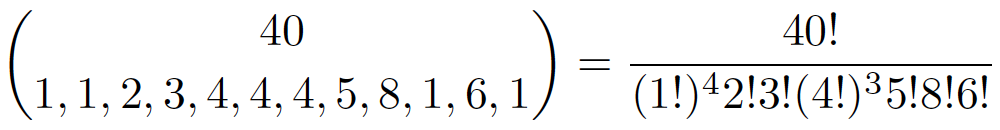
\includegraphics[width=1.0\linewidth]{fig01}
 \caption{Брой комбинации за първоначално подреждане на пионките \cite{arts01}}
\label{figure01}
\end{figure}
\FloatBarrier

\begin{lstlisting}
http://www.ultrastratego.com/setups.php
\end{lstlisting}

\subsection{Оптимално разиграване}

Голямо влияние върху развитието на играта оказват именно познанията и приложимостта  на различни стратегии от страна на играчите.

Позиция на флага:

Целта на играта е да бъде превзет противниковия флаг, за това отбраняването му е основна стратегия. Поставянето му в близост до ръбовете или ъглите, заграден с бомби го прави трудно  окупиран. Опонентът може да го достъпи само с помощта на миньор. Играчът може да  заблуди противника чрез поставяне на подобна структура, която защитава незначителна част по задната линия. По този начин, опонента изиграва повече ходове за да достигне флага.

Сапьорът:

Фигурата с най-висок ранг, която може да обърне играта в полза на играча. За целта участникът трябва да запази един от сапьорите си на игралното поле, докато не се увери, че е отстранил всички бомби от полето на опонента. По този начин може да превземе флага му и съответно да спечели играта.

Шпионинът:

Единствената подвижна пионка, която може да победи маршала, а той от своя страна се явява единствената подвижна пионка, която може да победи генерала. Ако генералът бъде победен от маршала ще бъде разкрит и шпионинът може да го победи, но трябва да бъде в близост до генерала, за предпочитане е съседна клетка. При първа възможност , шпионина веднага трябва  да атакува след поражението на генерала. И все пак, ако генералът обикаляше игралното поле със следваща го пионка, това е най-вероятно е шпионина.

\begin{figure}[h!]
 \centering
 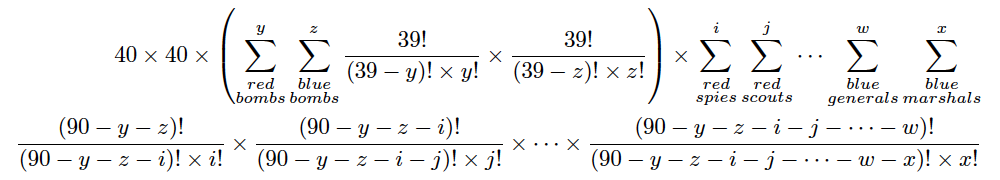
\includegraphics[width=1.0\linewidth]{fig02}
 \caption{Формула за възможните разигравания \cite{arts01}}
\label{figure02}
\end{figure}
\FloatBarrier

\begin{lstlisting}
http://www.ultrastratego.com/tactics.php
\end{lstlisting}

\section{Проблем, цели и задачи}

Логическите игри през вековете са имали за основна цел да развиват тактическите и стратегическите умения на различни хора в обществото (предимно военачалници). В наши дни логическите игри спомагат за развитие на умения при инвестиране или планиране. Също така логическите игри намират широко приложение като развлечение. С развитието на компютрите и мобилните устройства все повече класически игри (на дъска и не само) се реализират под формата на електронни игри и служат за уплътняване на свободното време. 

Настоящата дипломна работа адресира проблема свързан с развитието на логическото мислене при хората, на първо място и възможността за развлечения в моментите на скука, на второ място. 

Постигането на следните цели, поставени в дипломната работа водят до решаването на поставения проблем: \\
G.1 Разработка на електронна игра „Stratego“; \\
G.2 Разработка на възможности за реализация на изкуствен интелект в електронната игра; \\
G.3 Изследване на възможностите за различни стратегии;

Постигането на набелязаните в дипломната работа цели се осъществява, чрез изпълнението на следните задачи: \\
T.1.1 Изработване на графичен интерфейс за мобилно приложение на играта; \\
T.1.2 Изработване на обектно-ориентиран модел на електронната игра; \\
T.1.3 Изработване на релационен модел за съхраняване на информацията в играта; \\
Т.1.4 Изработване на програмен код за мобилна комуникация, така че играчите да имат възможност за игра в мрежа; \\
T.2.1 Съставяне на подходящи програмни модули за компютърен опонент; \\
T.2.2 Реализация на компютърен опонент по принципа „случайно търсене“ (Rrandom Search); \\
T.3.1 Реализация на изследване за оптимално първоначално подреждане на игралното табло с Монте Карло дървовидно търсене (Monte Carlo Tree Search); \\


\newpage
\chapter{Изработване на електронна игра}
\label{chapter02}

\section{Избор на развойни средства}

\section{Стратегии за проектиране}

\subsection{Трислоен софтуерен модел}

\begin{figure}[h!]
 \centering
 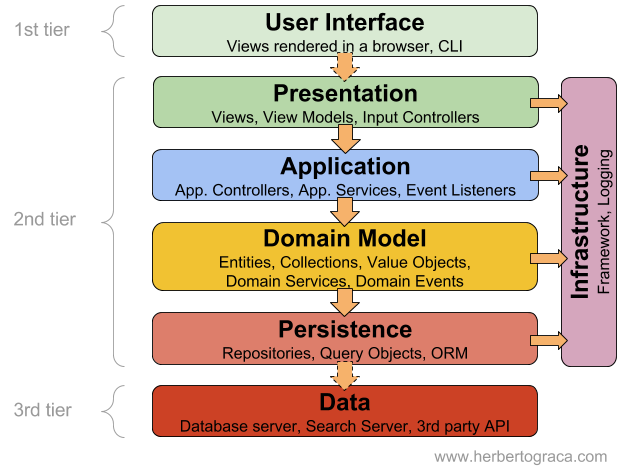
\includegraphics[width=1.0\linewidth]{fig03}
 \caption{Трислойна софтуерна архитектура}
\label{figure03}
\end{figure}
\FloatBarrier

\begin{lstlisting}
https://herbertograca.com/2017/08/03/layered-architecture/
\end{lstlisting}

\subsection{Подход отгоре на долу (Top-Down)}

\subsection{Подход отдоло на горе (Bottom-Up)}

\begin{lstlisting}
https://en.wikipedia.org/wiki/Top-down_and_bottom-up_design
\end{lstlisting}

 
%\include{chapters/chapter03}
%\include{chapters/chapter04} 
%\include{chapters/chapter05} 

%----------------------------------------------------------------------------------------
%   Приложения към основното изложени.
%----------------------------------------------------------------------------------------

\appendix

%\include{аppendices/аppendix01}
%\include{аppendices/аppendix02}
%\include{аppendices/аppendix03}

%----------------------------------------------------------------------------------------
%   Списък с използвана литература и източници на информация.
%----------------------------------------------------------------------------------------

\newpage
\begin{thebibliography}{99}

\bibitem{arts01} Arts, A.F.C.: Competitive Play in Stratego. In: Master Thesis DKE 10-05, Master of Science of Artificial Intelligence at the Faculty of Humanities and Sciences of Maastricht University, Netherlands (2010)

\end{thebibliography}

%----------------------------------------------------------------------------------------
%   Азбучен указател на използваните термини.
%----------------------------------------------------------------------------------------

\newpage
\printindex

\end{document}
